\documentclass[10pt,letterpaper,spanish,twoside]{report}

\usepackage{practica}
\usepackage{graphicx}
\usepackage{float}
\DeclareGraphicsExtensions{.bmp,.png,.pdf,.jpg}
\newcommand{\docdate}{
  \vspace{2em}
   \begin{flushright}
     Ciudad de México. \datedayname~\today.
   \end{flushright}
  \vspace{2em}
}

\begin{document}
\docdate

\begin{center}
 \textsc{\asignatura}\vspace{.2em}
\end{center}

\textsc{Manual del profesor}

\textsc{Práctica 6. aplicación de filtros digitales Chebyshev  tipo 1 y 2 rechaza banda a señales biomédicas reales}

\textsc{Objetivo:} Aplicar los conocimientos sobre el diseño de filtros digitales Cheyshev tipo 1 y 2 a señales biomédicas reales 

\textsc{Actividades}
\begin{enumerate}
 \item Se descarga el archivo 'PCG$\_$60.npz' de https://goo.gl/xCkryR
 \item Se recomienda reproducir la señal para identificar que efectivamente la señal se encuentra contaminada, se puede consultar el script 'P6$\_$FAyD' para realizar algún cambio en los filtros.\\En la figura~\ref{contexto:PCG} se muestra la señal de PCG
 \begin{figure}[H]
  \centering
  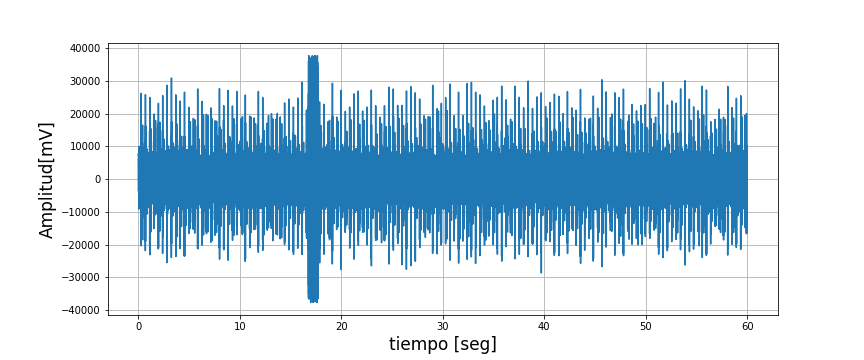
\includegraphics[scale=0.4]{PCG.PNG}
  \caption{Señal de PCG}
  \label{contexto:PCG}
 \end{figure}
 \item Obtener la FFT de la señal de forma digital, en la figura~\ref{contexto:FFT_PCG} se puede observar que la interferencia de la señal se encuentra en los 60 Hz.
 \begin{figure}[H]
  \centering
  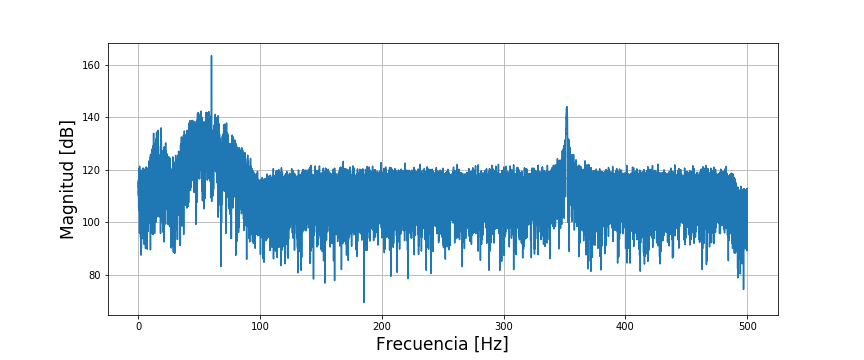
\includegraphics[scale=0.4]{FFT_c.PNG}
  \caption{FFT de señal de PCG}
  \label{contexto:FFT_PCG}
 \end{figure}
 \item Para el diseño del filtro digital tipo Chebyshev rechaza banda orden 4 tipo 1 se recomienda utilizar frecuencias de corte de 58 y 62 Hz. En la figura~\ref{contexto:RF_Cheby1PCG} se observa la respuesta en frecuencia del filtro, los puntos rojos muestran las frecuencias de corte, teniendo una caída de -3dB
 \begin{figure}[H]
  \centering
  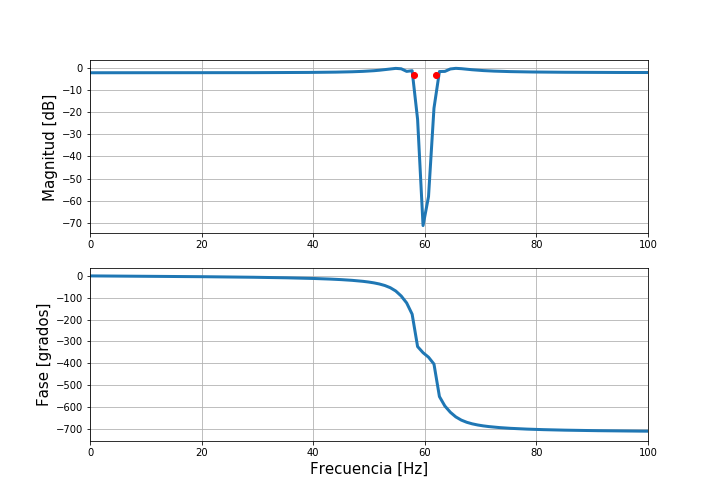
\includegraphics[scale=0.4]{RF_Cheby1PCG.PNG}
  \caption{Respuesta en frecuencia del filtro Chebyshev orden 4 tipo 1}
  \label{contexto:RF_Cheby1PCG}
 \end{figure}
 \item Se procede a realizar el filtrado de la señal en fase cero. En la figura~\ref{contexto:FFT_Cheby1PCG} se observa la FFT de la señal filtrada con un filtro Chebyshev tipo 1.\\Se puede observar que el ruido de 60 Hz fue eliminado correctamente, para poder evaluar el filtro se sugiere reproducir la señal filtrada.
 \begin{figure}[H]
  \centering
  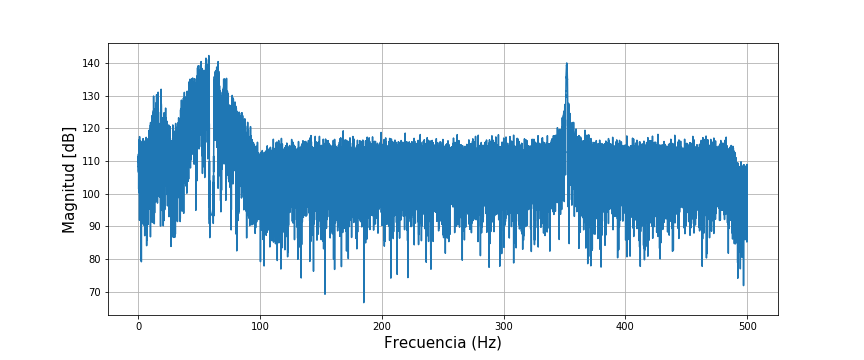
\includegraphics[scale=0.4]{FFT_Cheby1PCG.PNG}
  \caption{FFT de la señal filtrada con filtro Chebyshev orden 4 tipo 1}
 \label{contexto:FFT_Cheby1PCG}
 \end{figure}   
 \item Para el diseño del filtro Chebyshev orden 4 tipo 2 se recomiendan frecuencias de corte de 58.5 y 61.5 Hz. En la figura~\ref{contexto:RF_Cheby2PCG} se muestra la respuesta en frecuencia del filtro.
 \begin{figure}[H]
  \centering
  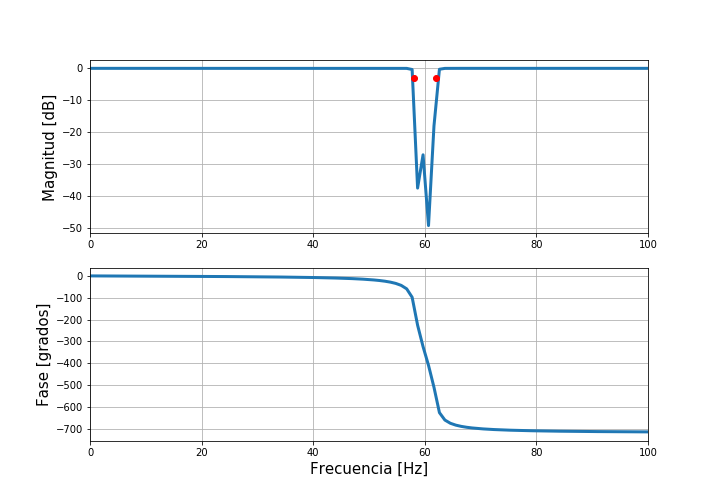
\includegraphics[scale=0.4]{RF_Cheby2PCG.PNG}
  \caption{Respuesta en frecuencia de filtro rechaza banda Chebyshev orden 4 tipo 2}
  \label{contexto:RF_Cheby2PCG}
 \end{figure}
 \item Se realiza el filtrado de la señal en fase cero. Para una mejor evaluación del funcionamiento del filtro se recomienda reproducir la señal filtrada\\En la figura~\ref{contexto:FFT_Cheby2PCG} se muestra la FFT de la señal filtrada, es posible observar que se elimina correctamente el ruido de 60 Hz.
 \begin{figure}[H]
  \centering
  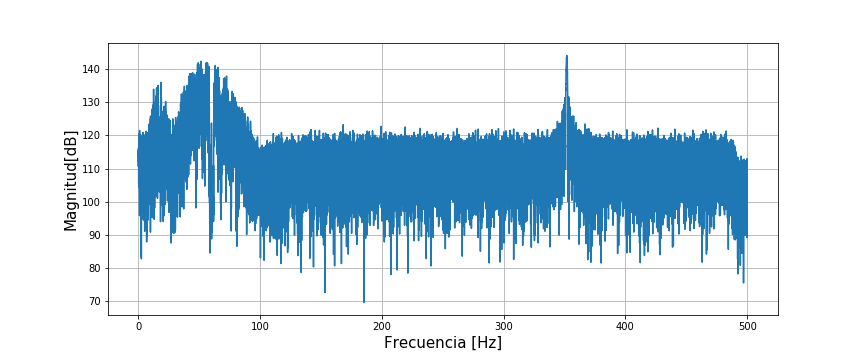
\includegraphics[scale=0.4]{FFT_Cheby2PCG.PNG}
  \caption{FFT de la señal filtrada con filtro CHebyshev orden 4 tipo 1}
  \label{contexto:FFT_Cheby2PCG} 
 \end{figure}
 \item Se puede realizar una comparación entre la FFT de las señales filtradas de la figura~\ref{contexto:FFT_Cheby1PCG} y \ref{contexto:FFT_Cheby2PCG} con la FFT de la señal original de la figura~\ref{contexto:FFT_PCG} observando que con ambos filtros es posible eliminar el ruido de 60 Hz utilizando frecuencias de corte distintas. Para una mejor evaluación se sugiere reproducir ambas señales filtradas.
\end{enumerate}

%\textsc{Nota}
%\vspace{2em}
\vfill
\begin{flushright}
\textsc{Elaboró:\\
Ma. del Rosario Aguilar Cruz\\
Enrique Mena Camilo}
\end{flushright}

\end{document}